\documentclass[10pt, aspectratio=169]{beamer}
\usefonttheme{professionalfonts}

\mode<presentation>
{
  \usetheme{Berkeley}
  \usecolortheme{beaver}
  \usefonttheme{default}
  \setbeamertemplate{navigation symbols}{}
  \setbeamertemplate{caption}[numbered]
} 

\setbeamertemplate{footline}{%
  \leavevmode%
  \hbox{%
    \begin{beamercolorbox}[wd=.85\paperwidth,ht=2.5ex,dp=1ex,left]{author in head/foot}%
      \usebeamerfont{author in head/foot}Maxx Seminario, Electronic Circuits, Fall 2025%
    \end{beamercolorbox}%
    \begin{beamercolorbox}[wd=.15\paperwidth,ht=2.5ex,dp=1ex,right]{date in head/foot}%
      \hspace*{0.5em}\insertframenumber{} / \inserttotalframenumber\hspace*{0.5em}%
    \end{beamercolorbox}%
  }%
  \vskip0pt%
}

\usepackage[english]{babel}
\usepackage[utf8x]{inputenc}
\usepackage{tikz}
\usetikzlibrary{shapes.geometric}
\usepackage{pgfplots}
\usepackage{array}
\usepackage{makecell}
\usepackage{verbatim}
\usepackage{graphicx}
\usepackage{subcaption}
\usepackage{amsfonts}
\usepackage{amsmath}
\usepackage{bm}
\usepackage{epstopdf}
\usepackage{circuitikz}
\usepackage{caption}
\captionsetup{compatibility=false}
\usepackage[absolute,overlay]{textpos}
\usetikzlibrary{calc}
\usetikzlibrary{pgfplots.fillbetween, backgrounds}
\usetikzlibrary{positioning}
\usetikzlibrary{pgfplots.groupplots}
\usetikzlibrary{plotmarks}
\usetikzlibrary{calc}
\usepgfplotslibrary{groupplots}
\pgfplotsset{compat=newest} 

\usepackage{hyperref}
\definecolor{BeaverRed}{RGB}{179,38,38} 
\hypersetup{
    colorlinks=true,
    linkcolor=BeaverRed,
    filecolor=magenta,      
    urlcolor=cyan,
}

% Added by Maxx Seminario 01/06/2026 - for colored icons in itemize labels
\usepackage{wasysym} % for smiles and frowns
\newcommand{\neutralface}{%
  \tikz[baseline=-0.6ex]{
    \draw (0,0) circle (0.9ex);
    \fill (-0.35ex,0.25ex) circle (0.12ex);
    \fill ( 0.35ex,0.25ex) circle (0.12ex);
    \draw (-0.35ex,-0.25ex) -- (0.35ex,-0.25ex);
  }%
}

\newcommand{\baditem}{\textcolor{red!70!black}{\frownie}}
\newcommand{\gooditem}{\textcolor{green!60!black}{\smiley}}
\newcommand{\mehitem}{\textcolor{orange!80!black}{\neutralface}}


% =========================
% Solution toggle 
% =========================
\newif\ifshowsolutions
\showsolutionstrue   %  compile WITH solutions
%\showsolutionsfalse %  compile WITHOUT solutions



% =========================
% Document Information
% =========================
\title[The Ideal Op-Amp]{The Ideal Operational Amplifier}
\subtitle{Op-Amp Fundamentals and Characteristics}
\author{Maxx Seminario}
\institute{University of Nebraska-Lincoln}
\date{Spring 2026}

\begin{document}

\begin{frame}
  \titlepage
\end{frame}

\begin{frame}{Outline}
  \tableofcontents
\end{frame}

\section{Introduction to the Op-Amp}

\begin{frame}{What is an Operational Amplifier?}
    
    \begin{columns}[t]
    \column{0.48\textwidth}
        \textbf{The Op-Amp}: 
        \begin{itemize}
            \item High-gain differential amplifier
            \item Integrated circuit (IC) device
            \item Versatile building block
            \item Typcially used in feedback
        \end{itemize}
        
        \vspace{0.4cm}
        
        \textbf{Key Applications}:
        \begin{itemize}
            \item Signal amplification
            \item Filtering
            \item Mathematical operations
            \item Signal conditioning
            \item Analog computation
        \end{itemize}
        
    \column{0.48\textwidth}
        \begin{figure}[htb]
        \centering
        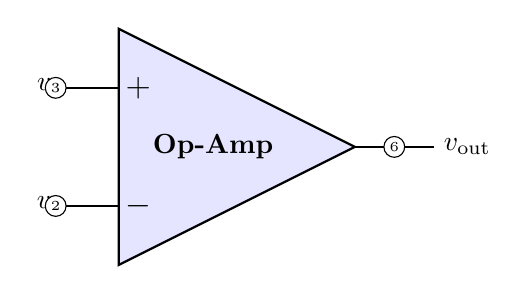
\begin{tikzpicture}[scale=1.0]
        % Op-amp triangle pointing right (tip at x=3)
        \draw[fill=blue!10, thick] (0,-1.5) -- (0,1.5) -- (3,0) -- cycle;

        % Input terminals on the left
        \draw[thick] (-0.8,0.75) -- (0,0.75) node[left, xshift=-0.5cm] {$v_+$}; % non-inverting
        \draw[thick] (-0.8,-0.75) -- (0,-0.75) node[left, xshift=-0.5cm] {$v_-$}; % inverting

        % Plus/minus labels near the left edge of the triangle
        \node at (0.25,0.75) {\large $+$};
        \node at (0.25,-0.75) {\large $-$};

        % Output terminal on the right
        \draw[thick] (3,0) -- (4,0) node[right] {$v_{\text{out}}$};

        % Optional terminal numbers
        \node[fill=white, circle, draw, inner sep=1pt] at (-0.8,0.75) {\tiny 3}; % non-inverting input
        \node[fill=white, circle, draw, inner sep=1pt] at (-0.8,-0.75) {\tiny 2}; % inverting input
        \node[fill=white, circle, draw, inner sep=1pt] at (3.5,0) {\tiny 6}; % output

        % Label
        \node at (1.2,0) {\textbf{Op-Amp}};
        \end{tikzpicture}
  
        \caption{Op-amp circuit symbol}
        \end{figure}
        
        \vspace{-0.2cm}
        
        \begin{block}{Black Box Approach}
            We treat the op-amp as a \textbf{black box} with well-defined terminal behavior
        \end{block}
        
    \end{columns}
    
\end{frame}

\begin{frame}{Op-Amp Terminals}
    
    \begin{columns}[t]
    \column{0.48\textwidth}
        \textbf{Signal Terminals} (3):
        \begin{enumerate}
            \item \textbf{Inverting input} $(-)$:  Terminal 1
            \item \textbf{Noninverting input} $(+)$: Terminal 2
            \item \textbf{Output}:  Terminal 3
        \end{enumerate}
        
        \vspace{0.3cm}
        
        \textbf{Power Supply Terminals} (2):
        \begin{itemize}
            \item Terminal 4: $+V_{CC}$ (positive supply)
            \item Terminal 5: $-V_{EE}$ (negative supply)
        \end{itemize}
        
        \vspace{0.3cm}
        
        \textbf{Other Terminals}:
        \begin{itemize}
            \item Frequency compensation
            \item Offset nulling
            \item (Application specific)
        \end{itemize}
        
    \column{0.48\textwidth}
        \begin{figure}[htb]
        \centering
        \begin{circuitikz}[scale=1.0]
            % Op-amp with power supplies
            \draw (0,0) node[op amp, scale=1.5] (opamp) {};
            
            % Input labels
            \node at (opamp.-) [left, yshift=6pt] {\small 1};
            \node at (opamp.+) [left, yshift=6pt] {\small 2};
            \node at (opamp.out) [right, yshift=6pt] {\small 3};
            
            % Power supply connections
            \draw (opamp.up) -- ++(0,0.5) node[above] {\small 4: $+V_{CC}$};
            \draw (opamp.down) -- ++(0,-0.5) node[below] {\small 5: $-V_{EE}$};
            
            % Input signals
            \draw (opamp.-) -- ++(-0.8,0) node[left] {$v_1$};
            \draw (opamp.+) -- ++(-0.8,0) node[left] {$v_2$};
            
            % Output signal
            \draw (opamp.out) -- ++(0.8,0) node[right] {$v_3$};
        \end{circuitikz}
        \caption{Op-amp with all terminals shown}
        \end{figure}
    
        
    \end{columns}
    
\end{frame}

\section{Ideal Op-Amp Characteristics}

% \begin{frame}{The Ideal Op-Amp Small-Signal Model}
%   \begin{figure}[htb]
%     \centering
%     \begin{tikzpicture}[scale=1, >=stealth]
      
%       % Op-amp triangle (dashed outline)
%       \draw[line width=1.5pt, dashed] (2,3) -- (9,0) -- (2,-3) -- cycle;
      
%       % Dashed vertical line at inputs
%       \draw[line width=1.5pt, dashed] (2,3) -- (2,-3);
      
%       % Input terminal 1 (top)
%       \draw[line width=0.8pt] (0,2) -- (2,2);
%       \node at (0.3,2) {\small $\circ$};
%       \node[left] at (0,2) {1};
%       \node at (1.8,2) {\small $\circ$};
      
%       % Input terminal 2 (bottom)
%       \draw[line width=0.8pt] (0,-2) -- (2,-2);
%       \node at (0.3,-2) {\small $\circ$};
%       \node[left] at (0,-2) {2};
%       \node at (1.8,-2) {\small $\circ$};
      
%       % Output terminal 3
%       \draw[line width=0.8pt] (9,0) -- (10,0);
%       \node at (9.3,0) {\small $\circ$};
%       \node[right] at (10,0) {3};
      
%       % v1 voltage source (terminal 1)
%       \node at (1.2,2.3) {$+$};
%       \node at (1.2,1.7) {$v_1$};
%       \node at (1.2,1.4) {$-$};
      
%       % Ground for v1
%       \draw[line width=0.8pt] (1.2,1.2) -- (1.2,0.9);
%       \draw[line width=0.8pt] (1.0,0.9) -- (1.4,0.9);
%       \draw[line width=0.8pt] (1.1,0.75) -- (1.3,0.75);
%       \draw[line width=0.8pt] (1.15,0.62) -- (1.25,0.62);
      
%       % Current source Gm*v1 (diamond)
%       \draw[line width=0.8pt] (3,1.5) -- (3.3,1.2) -- (3,0.9) -- (2.7,1.2) -- cycle;
%       \draw[->, line width=0.8pt] (3,1.35) -- (3,1.05);
%       \node[right] at (3.3,1.2) {$G_m v_1$};
      
%       % Ground for Gm*v1
%       \draw[line width=0.8pt] (3,0.7) -- (3,0.4);
%       \draw[line width=0.8pt] (2.8,0.4) -- (3. 2,0.4);
%       \draw[line width=0.8pt] (2.9,0.25) -- (3.1,0.25);
%       \draw[line width=0.8pt] (2.95,0.12) -- (3.05,0.12);
      
%       % v2 voltage source (terminal 2)
%       \node at (1.2,-1.7) {$+$};
%       \node at (1.2,-2.3) {$v_2$};
%       \node at (1.2,-2.6) {$-$};
      
%       % Ground for v2
%       \draw[line width=0.8pt] (1.2,-2.8) -- (1.2,-3.1);
%       \draw[line width=0.8pt] (1.0,-3.1) -- (1.4,-3.1);
%       \draw[line width=0.8pt] (1.1,-3.25) -- (1.3,-3.25);
%       \draw[line width=0.8pt] (1.15,-3.38) -- (1.25,-3.38);
      
%       % Current source Gm*v2 (diamond)
%       \draw[line width=0.8pt] (3,-0.9) -- (3.3,-1.2) -- (3,-1.5) -- (2.7,-1.2) -- cycle;
%       \draw[->, line width=0.8pt] (3,-1.05) -- (3,-1.35);
%       \node[right] at (3.3,-1.2) {$G_m v_2$};
      
%       % Ground for Gm*v2
%       \draw[line width=0.8pt] (3,-1.7) -- (3,-2.0);
%       \draw[line width=0.8pt] (2.8,-2.0) -- (3.2,-2.0);
%       \draw[line width=0.8pt] (2.9,-2.15) -- (3.1,-2.15);
%       \draw[line width=0.8pt] (2.95,-2.28) -- (3.05,-2.28);
      
%       % Connection to resistor R
%       \draw[line width=0.8pt] (4. 5,1.5) -- (4.5,0.5);
%       \draw[line width=0.8pt] (4.5,-1.5) -- (4.5,-0.5);
%       \draw[line width=0.8pt] (3.3,1.2) -- (4.5,1.2);
%       \draw[line width=0.8pt] (3.3,-1.2) -- (4.5,-1.2);
      
%       % Resistor R (rectangular shape)
%       \draw[line width=0.8pt] (4.2,0.5) rectangle (4.8,-0.5);
%       \node at (4.5,0) {$R$};
      
%       % vd voltage label and markers
%       \node at (5.2,0.3) {$+$};
%       \node[right] at (5.4,0) {$v_d$};
%       \node at (5.2,-0.3) {$-$};
%       \node at (5.0,0.5) {\small $\circ$};
%       \node at (5.0,-0.5) {\small $\circ$};
      
%       % Ground for vd
%       \draw[line width=0.8pt] (4.5,-0.7) -- (4.5,-1.0);
%       \draw[line width=0.8pt] (4.3,-1.0) -- (4.7,-1.0);
%       \draw[line width=0.8pt] (4.4,-1.15) -- (4.6,-1.15);
%       \draw[line width=0.8pt] (4.45,-1.28) -- (4.55,-1.28);
      
%       % Dependent voltage source μ*vd (diamond)
%       \draw[line width=0.8pt] (6.5,0.4) -- (6.8,0.1) -- (6.5,-0.2) -- (6.2,0.1) -- cycle;
%       \node at (6.5,0.25) {\small $+$};
%       \node at (6.5,-0.05) {\small $-$};
%       \node[right] at (6.8,0.1) {$\mu v_d$};
      
%       % Connection from vd to μ*vd
%       \draw[line width=0.8pt] (5.0,0.5) -- (6.5,0.5) -- (6.5,0.4);
      
%       % Ground for μ*vd
%       \draw[line width=0.8pt] (6.5,-0.4) -- (6.5,-0.7);
%       \draw[line width=0.8pt] (6.3,-0.7) -- (6.7,-0.7);
%       \draw[line width=0.8pt] (6.4,-0.85) -- (6.6,-0.85);
%       \draw[line width=0.8pt] (6.45,-0.98) -- (6.55,-0.98);
      
%       % Connection to output
%       \draw[line width=0.8pt] (6.5,0.4) -- (6.5,0.8) -- (9,0.8) -- (9,0);
      
%       % Output terminal markings
%       \node at (9.3,0.3) {$+$};
%       \node at (9.3,-0.3) {$v_3$};
%       \node at (9.3,-0.6) {$-$};
      
%       % Ground at output
%       \draw[line width=0.8pt] (9. 5,-0.8) -- (9.5,-1.1);
%       \draw[line width=0.8pt] (9.3,-1.1) -- (9.7,-1.1);
%       \draw[line width=0.8pt] (9.4,-1.25) -- (9.6,-1.25);
%       \draw[line width=0.8pt] (9.45,-1.38) -- (9.55,-1.38);
      
%     \end{tikzpicture}
%     \caption{Small-signal op-amp model}
%     \label{fig: opamp_small_signal}
%   \end{figure}
% \end{frame}

\begin{frame}{Five Characteristics of the Ideal Op-Amp}
  \begin{itemize}
    \setlength{\itemsep}{4pt} 
    \item \textbf{Infinite input impedance} ($Z_{in} \to \infty$) $\rightarrow$ $i_1 = i_2 = 0$
    \item \textbf{Zero output impedance} ($Z_{out} = 0$) $\rightarrow$ ideal voltage source at output
    \item \textbf{Infinite open-loop gain} ($A \to \infty$) $\rightarrow$ tiny $(v_2 - v_1)$ produces large $v_3$
    \item \textbf{Infinite bandwidth} $\rightarrow$ flat gain from DC to $\infty$
    \item \textbf{Zero common-mode gain} (infinite CMRR) $\rightarrow$ responds only to differential input
  \end{itemize}

  \begin{block}{Important}
    These are idealizations; real op-amps approximate them, and designs must account for non-idealities.
  \end{block}
\end{frame}


\begin{frame}{Op-Amp Circuit Symbol with Ideal Assumptions}
  \begin{figure}[htb]
    \centering
    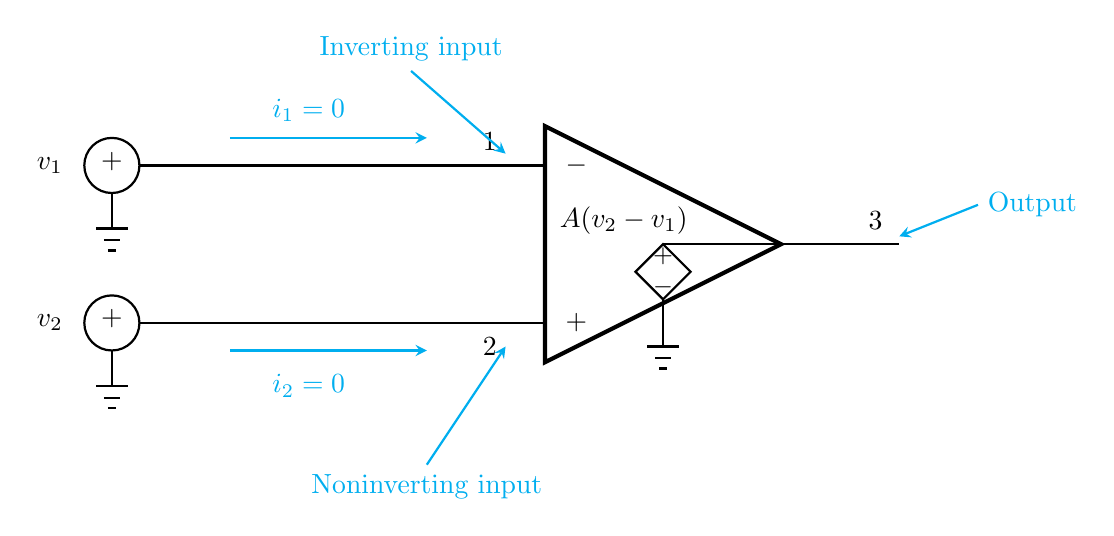
\begin{tikzpicture}[scale=1, >=stealth]
      % Define colors
      \definecolor{labelcyan}{RGB}{0, 174, 239}
      
      % Op-amp triangle
      \draw[line width=1.5pt] (4,1.5) -- (7,0) -- (4,-1.5) -- cycle;
      
      % Connection lines
      \draw[line width=0.8pt] (0.  5,1) -- (4,1);
      \draw[line width=0.8pt] (0.5,-1) -- (4,-1);
      \draw[line width=0.8pt] (7,0) -- (8.  5,0);
      
      % Terminal symbols (- and +)
      \node at (4.  4,1) {$-$};
      \node at (4.4,-1) {$+$};
      
      % Terminal numbers
      \node at (3.3,1.3) {1};
      \node at (3.3,-1.3) {2};
      \node at (8.2,0.3) {3};
      
      % Voltage source v1 (inverting input)
      \draw[line width=0.8pt] (-1.5,1) circle (0.35);
      \node at (-1.5,1.05) {$+$};
      \node[left] at (-2,1) {$v_1$};
      \draw[line width=0.8pt] (-1.15,1) -- (0.5,1);
      
      % Ground for v1
      \draw[line width=0.8pt] (-1.5,0.65) -- (-1.5,0.2);
      \draw[line width=0.8pt] (-1.7,0.2) -- (-1.3,0.2);
      \draw[line width=0.8pt] (-1.6,0.05) -- (-1.4,0.05);
      \draw[line width=0.8pt] (-1.55,-0.08) -- (-1.45,-0.08);
      
      % Voltage source v2 (noninverting input)
      \draw[line width=0.8pt] (-1.5,-1) circle (0.35);
      \node at (-1.5,-0.95) {$+$};
      \node[left] at (-2,-1) {$v_2$};
      \draw[line width=0.8pt] (-1.15,-1) -- (0.5,-1);
      
      % Ground for v2
      \draw[line width=0.8pt] (-1.5,-1.35) -- (-1.5,-1.8);
      \draw[line width=0.8pt] (-1.7,-1.8) -- (-1.3,-1.8);
      \draw[line width=0.8pt] (-1.6,-1.95) -- (-1.4,-1.95);
      \draw[line width=0.8pt] (-1.55,-2.08) -- (-1.45,-2.08);
      
      % Current annotations (i1 = 0, i2 = 0)
      \draw[->, labelcyan, line width=0.8pt] (0,1.35) -- (2.5,1.35);
      \node[labelcyan] at (1,1.7) {$i_1 = 0$};
      
      \draw[->, labelcyan, line width=0.8pt] (0,-1.35) -- (2.5,-1.35);
      \node[labelcyan] at (1,-1.8) {$i_2 = 0$};
      
      % Dependent voltage source (diamond shape)
      \draw[line width=0.8pt] (5.5,0) -- (5.85,-0.35) -- (5.5,-0.7) -- (5.15,-0.35) -- cycle;
      \node at (5.5,-0.15) {\small $+$};
      \node at (5.5,-0.55) {\small $-$};
      
      % Connection from top of diamond to op-amp output
      \draw[line width=0.8pt] (5.5,0) -- (7,0);
      
      % A(v2-v1) label
      \node[below] at (5,0.6) {$A(v_2 - v_1)$};
      
      % Ground at power supply
      \draw[line width=0.8pt] (5.5,-0.7) -- (5.5,-1.3);
      \draw[line width=0.8pt] (5.3,-1.3) -- (5.7,-1.3);
      \draw[line width=0.8pt] (5.4,-1.45) -- (5.6,-1.45);
      \draw[line width=0.8pt] (5.45,-1.58) -- (5.55,-1.58);
      
      % Labels with arrows
      \draw[->, labelcyan, line width=0.8pt] (2.3,2.2) -- (3.5,1.15);
      \node[labelcyan, above] at (2.3,2.2) {Inverting input};
      
      \draw[->, labelcyan, line width=0.8pt] (2.5,-2.8) -- (3.5,-1.3);
      \node[labelcyan, below] at (2.5,-2.8) {Noninverting input};
      
      \draw[->, labelcyan, line width=0.8pt] (9.5,0.5) -- (8.5,0.1);
      \node[labelcyan, right] at (9.5,0.5) {Output};
      
    \end{tikzpicture}
    \caption{Equivalent Circuit for Ideal Op-Amp}
    \label{fig: opamp_small_signal}
  \end{figure}
\end{frame}


\begin{frame}{Inverting vs.  Noninverting Inputs}
    
    \begin{columns}[t]
    \column{0.48\textwidth}
        \textbf{Inverting Input} $(-)$:
        \begin{itemize}
            \item Output is \textbf{out of phase}
            \item Signal inverted (180° phase shift)
        \end{itemize}
        
        % \vspace{0.3cm}
        
        \begin{figure}[htb]
        \centering
        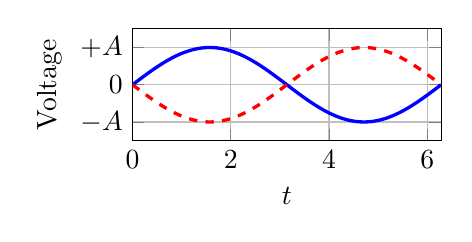
\begin{tikzpicture}
            \begin{axis}[
                width=5.5cm, height=3cm,
                xlabel={$t$},
                ylabel={Voltage},
                domain=0:2*pi,
                samples=100,
                grid=major,
                xmin=0, xmax=2*pi,
                ymin=-1.5, ymax=1.5,
                legend pos=north east,
                xtick={},
                ytick={-1,0,1},
                yticklabels={$-A$, 0, $+A$},
            ]
            
            \addplot[blue, very thick] {sin(deg(x))};
            % \addlegendentry{$v_1$ (input)}
            
            \addplot[red, very thick, dashed] {-sin(deg(x))};
            % \addlegendentry{$v_3$ (output)}
            
            \end{axis}
        \end{tikzpicture}
        \caption{Inverting input response}
        \end{figure}
        
    \column{0.48\textwidth}
        \textbf{Noninverting Input} $(+)$:
        \begin{itemize}
            \item Output is \textbf{in phase}
            \item Signal not inverted (0° phase shift)
        \end{itemize}
        
        % \vspace{0.3cm}
        
        \begin{figure}[htb]
        \centering
        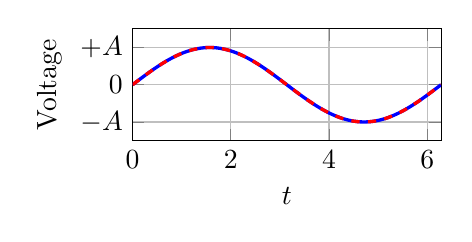
\begin{tikzpicture}
            \begin{axis}[
                width=5.5cm, height=3cm,
                xlabel={$t$},
                ylabel={Voltage},
                domain=0:2*pi,
                samples=100,
                grid=major,
                xmin=0, xmax=2*pi,
                ymin=-1.5, ymax=1.5,
                legend pos=north east,
                xtick={},
                ytick={-1,0,1},
                yticklabels={$-A$, 0, $+A$},
            ]
            
            \addplot[blue, very thick] {sin(deg(x))};
            % \addlegendentry{$v_2$ (input)}
            
            \addplot[red, very thick, dashed] {sin(deg(x))};
            % \addlegendentry{$v_3$ (output)}
            
            \end{axis}
        \end{tikzpicture}
        \caption{Noninverting input response}
        \end{figure}
        
    \end{columns}
    
    \vspace{0.3cm}
    
    \begin{block}{Remember}
        Output:  $v_3 = A(v_2 - v_1)$ — noninverting term $(+v_2)$, inverting term $(-v_1)$
    \end{block}
    
\end{frame}


\section{Differential and Common-Mode Signals}

\begin{frame}{Differential-Input, Single-Ended Output}
    
    \begin{columns}[t]
    \column{0.48\textwidth}
        \textbf{Differential Input}:
        \[
        v_{Id} = v_2 - v_1
        \]
        
        \begin{itemize}
            \item The \textbf{difference} between inputs
            \item What the op-amp amplifies
        \end{itemize}
        
        \textbf{Common-Mode Input}:
        \[
        v_{Icm} = \frac{1}{2}(v_1 + v_2)
        \]
        
        \begin{itemize}
            \item The \textbf{average} of inputs
            \item Ideally \textbf{rejected} by op-amp
            \item Noise component (often)
        \end{itemize}
        
    \column{0.48\textwidth}
        \begin{figure}[htb]
        \centering
        \begin{circuitikz}[scale=0.9]
            % Two voltage sources
            \draw (0,2) to[sV, l=$v_{Icm} + \frac{v_{Id}}{2}$] (0,0);
            \draw (0,0) node[ground] {};
            \draw (0,2) to[short, -o] (1,2) node[right] {$v_2$};
            
            \draw (0,-1) to[sV, l=$v_{Icm} - \frac{v_{Id}}{2}$] (0,-3);
            \draw (0,-3) node[ground] {};
            \draw (0,-1) to[short, -o] (1,-1) node[right] {$v_1$};
            
            % Labels
            \node[blue] at (-1.5,2) {Noninverting};
            \node[blue] at (-1.5,-1) {Inverting};
        \end{circuitikz}
        \caption{Signal decomposition}
        \end{figure}
        
    \end{columns}
    
    \vspace{0.2cm}
    
    \begin{block}{Ideal Op-Amp Behavior}
        Infinite common-mode rejection $\rightarrow$ Output depends \textbf{only} on $v_{Id} = v_2 - v_1$
    \end{block}
    
\end{frame}

\begin{frame}{Common-Mode Rejection}
    
    \begin{columns}[t]
    \column{0.48\textwidth}
        \textbf{Why Common-Mode Rejection?}
        \begin{itemize}
            \item Noise often appears equally on both inputs
            \item Power line interference
            \item Environmental pickup
            \item Ground potential differences
        \end{itemize}
        
        \vspace{0.3cm}
        
        \textbf{Ideal Op-Amp}:
        \begin{itemize}
            \item Common-mode gain = 0
            \item CMRR = $\infty$ dB
            \item Perfectly rejects $v_{Icm}$
        \end{itemize}
        
        
    \column{0.48\textwidth}
        \begin{figure}[htb]
        \centering
        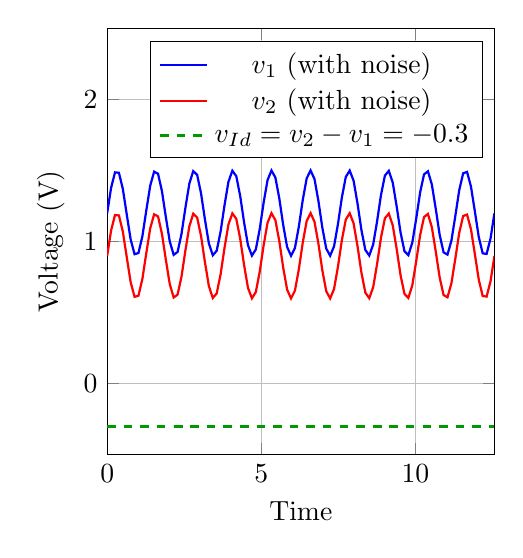
\begin{tikzpicture}
            \begin{axis}[
                width=6.5cm, height=7cm,
                xlabel={Time},
                ylabel={Voltage (V)},
                domain=0:4*pi,
                samples=100,
                grid=major,
                xmin=0, xmax=4*pi,
                ymin=-0.5, ymax=2.5,
                legend pos=north east,
                xtick={},
                ytick={0,1,2},
            ]
            
            % Noise on both inputs (common-mode)
            \addplot[blue, thick] {1.2 + 0.3*sin(deg(5*x))};
            \addlegendentry{$v_1$ (with noise)}
            
            \addplot[red, thick] {0.9 + 0.3*sin(deg(5*x))};
            \addlegendentry{$v_2$ (with noise)}
            
            % Differential output (noise cancelled)
            \addplot[green! 60!black, very thick, dashed] {-0.3};
            \addlegendentry{$v_{Id} = v_2 - v_1 = -0.3$}
            
            \end{axis}
        \end{tikzpicture}
        \caption{Common-mode noise rejection example}
        \end{figure}
        
    \end{columns}
    
\end{frame}

\section{Key Properties}

\begin{frame}{Open-Loop Gain:  Why Infinite? }
\begin{columns}[t]
  \begin{column}{0.48\textwidth}
    \textbf{Open-Loop Configuration}:
    \begin{itemize}
      \item No feedback from output to input
      \item Gain $A = \infty$ (ideal)
      \item \textbf{Not practical} 
    \end{itemize}

    \textbf{Why $A = \infty$?}
    \begin{itemize}
      \item With feedback, gain becomes predictable
      \item Allows precise closed-loop gain
      \item Makes circuits insensitive to $A$ variations
    \end{itemize}

    \begin{block}{Practical Note}
      Real op-amps:  $A \approx 10^3$ to $10^6$ (60 dB to 120 dB)
    \end{block}
  \end{column}

  \begin{column}{0.48\textwidth}
    \vspace{-0.5 cm} % ensures top alignment baseline
    \begin{figure}
      \centering
      \begin{circuitikz}[scale=1.0]
        % Open-loop op-amp
        \draw (0,0) node[op amp, yscale=1.5, xscale=1.5] (opamp) {};

        \draw (opamp.+) -- ++(-0.7,0) coordinate (vinstart);
        \draw (vinstart) to[sV, l=$v_{in}$] ++(0,-1) node[ground] {};

        % Inverting input to ground
        \draw (opamp.-) -- ++(-0.5,0) node[ground] {};

        % Output
        \draw (opamp.out) to[short, -o] ++(1,0) node[right] {$v_{out}$};

        % Equation
        \node at (1,-2) {$v_{out} = A \cdot v_{in}$};
      \end{circuitikz}
      \caption{Open-loop configuration (impractical)}
    \end{figure}

    \textbf{Problem with Open-Loop}:
    \begin{itemize}
      \item Unstable and unpredictable
      \item Sensitive to temperature, supply, etc.
    \end{itemize}
  \end{column}
\end{columns}
\end{frame}

\begin{frame}{DC Amplification and Bandwidth}
    
    \begin{columns}[t]
    \column{0.48\textwidth}
        \textbf{Direct-Coupled (DC) Amplifier}:
        \begin{itemize}
            \item Amplifies down to \textbf{0 Hz} (DC)
            \item No coupling capacitors needed
            \item Preserves DC level of signals
        \end{itemize}
        
        \textbf{Advantages}:
        \begin{itemize}
            \item Measure slow-varying signals
            \item Sensor interfaces
            \item Precision applications
        \end{itemize}
        
        \textbf{Disadvantages}:
        \begin{itemize}
            \item DC offsets can be problematic
            \item Drift with temperature
        \end{itemize}
        
    \column{0.48\textwidth}
        \textbf{Infinite Bandwidth (Ideal)}:

        \vspace{-0.4cm}
        
        \begin{figure}[htb]
        \centering
        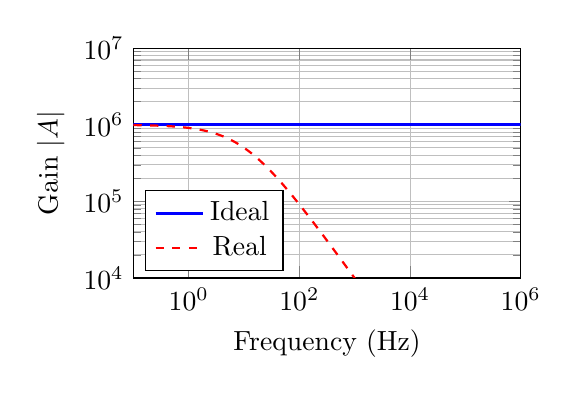
\begin{tikzpicture}
            \begin{axis}[
                width=6.5cm, height=4.5cm,
                xlabel={Frequency (Hz)},
                ylabel={Gain $|A|$},
                xmode=log,
                ymode=log,
                domain=0.1:1000000,
                samples=100,
                grid=both,
                xmin=0.1, xmax=1000000,
                ymin=1e4, ymax=1e7,
                legend pos=south west,
            ]
            
            % Ideal op-amp (flat response)
            \addplot[blue, very thick] {1e6};
            \addlegendentry{Ideal}
            
            % Real op-amp (with rolloff) - for comparison
            \addplot[red, thick, dashed] {1e6 / (1 + x/10)};
            \addlegendentry{Real}
            
            \end{axis}
        \end{tikzpicture}
        \caption{Ideal vs. real frequency response}
        \end{figure}
        
        \vspace{-0.4cm}
        
        \begin{itemize}
            \item Ideal: constant gain at all frequencies
            \item Real:  gain decreases at high frequency
        \end{itemize}
        
    \end{columns}
    
\end{frame}

\begin{frame}{Input and Output Impedances}
    
    \begin{columns}[t]
    \column{0.48\textwidth}
        \textbf{Infinite Input Impedance}:
        
        \begin{figure}[htb]
        \centering
        \begin{circuitikz}[scale=1.0]
            % Source with high impedance
            \draw (0,0) to[sV, l=$v_s$] (0,2);
            \draw (0,2) to[R, l=$R_s$] (2,2);
            \draw (0,0) -- (2,0);
            
            % Op-amp input (no current)
            \draw (2,2) to[short, -o] (3,2) node[right] {$v_{in}$};
            \draw (2,0) to[short, -o] (3,0);
            \draw[->, red, very thick] (2.5,2.3) -- (2.5,2.8) node[above] {$i = 0$};
            
            % Equation
            \node at (1.5,-0.8) {$v_{in} = v_s$ (no drop!)};
        \end{circuitikz}
        \caption{Input:  no loading effect}
        \end{figure}
        
        \vspace{0.2cm}
        
        \textbf{Benefit}:
        \begin{itemize}
            \item No loading of source
            \item $v_{in} = v_s$ regardless of $R_s$
        \end{itemize}
        
    \column{0.48\textwidth}
        \textbf{Zero Output Impedance}:
        
        \begin{figure}[htb]
        \centering
        \begin{circuitikz}[scale=1.0]
            % Op-amp output (ideal voltage source)
            \draw (0,0) to[sV, l=$A v_{in}$] (0,2);
            \draw (0,2) -- (1,2);
            \draw (0,0) -- (1,0);
            
            % Load
            \draw (1,2) to[R, l=$R_L$, v^>=$v_o$] (1,0);
            
            % Equation
            \node at (0.5,-0.8) {$v_o = A v_{in}$ (any $R_L$!)};
        \end{circuitikz}
        \caption{Output: ideal voltage source}
        \end{figure}
        
        \vspace{0.2cm}
        
        \textbf{Benefit}:
        \begin{itemize}
            \item Output voltage independent of load
            \item Can drive any $R_L$
        \end{itemize}
        
    \end{columns}
    
    \vspace{0.3cm}
    
    \begin{block}{Ideal Conditions}
        $Z_{in} = \infty \Rightarrow i_1 = i_2 = 0$ \quad and \quad $Z_{out} = 0 \Rightarrow v_o$ constant (any load)
    \end{block}
    
\end{frame}

\section{Summary and Examples}

\begin{frame}{Summary:  The Ideal Op-Amp}
    
    \begin{columns}[t]
    \column{0.48\textwidth}
        \textbf{Five Golden Rules}: 
        \begin{enumerate}
            \item $Z_{in} = \infty$ (no input current)
            \item $Z_{out} = 0$ (ideal voltage source)
            \item $A = \infty$ (infinite gain)
            \item Infinite bandwidth (DC to $\infty$)
            \item Infinite CMRR (rejects common-mode)
        \end{enumerate}
        
        \vspace{0.3cm}
        
        \textbf{Key Relationships}:
        \begin{itemize}
            \item $v_3 = A(v_2 - v_1)$
            \item $i_1 = i_2 = 0$
            \item $v_{Id} = v_2 - v_1$
            \item $v_{Icm} = \frac{1}{2}(v_1 + v_2)$
        \end{itemize}
        
    \column{0.48\textwidth}
        \begin{figure}[htb]
        \centering
        \begin{circuitikz}[scale=1.1]
            % Complete ideal op-amp
            \draw (0,0) node[op amp, yscale=1.5] (opamp) {};
            
            % Labels
            \node at (opamp.-) [left, xshift=-0.3cm] {$v_1$};
            \node at (opamp.+) [left, xshift=-0.3cm] {$v_2$};
            \node at (opamp.out) [right, xshift=0.3cm] {$v_3$};
            
            % Current annotations - horizontal arrows
            \draw[->, red, thick] ([xshift=-1.2cm, yshift=0.3cm]opamp.-) -- ([xshift=-0.1cm, yshift=0.3cm]opamp.-) node[midway, above] {$i_1=0$};
            \draw[->, red, thick] ([xshift=-1.2cm, yshift=0.3cm]opamp.+) -- ([xshift=-0.1cm, yshift=0.3cm]opamp.+) node[midway, above] {$i_2=0$};
                
            % Gain annotation
            \node[align=center, blue] at (0,-2.2) {$v_3 = A(v_2-v_1)$\\$A = \infty$};
        \end{circuitikz}
        \caption{Ideal op-amp summary}
        \end{figure}
        
    \end{columns}
    
\end{frame}

\begin{frame}{Practice Problem 1}
    \textbf{Measurements}:
    \begin{itemize}
        \item[(a)] $v_2 = 0$ V and $v_3 = 2$ V
        \item[(b)] $v_2 = +5$ V and $v_3 = -10$ V
        \item[(c)] $v_1 = 1.002$ V and $v_2 = 0.998$ V
    \end{itemize}

    \vspace{0.3cm}

    \textbf{Find}: The missing terminal voltage, $v_{Id}$, and $v_{Icm}$ for each case.

    \vspace{0.5cm}

    \textbf{Hints}:
    \begin{itemize}
        \item Use $v_3 = A(v_2 - v_1)$
        \item $v_{Id} = v_2 - v_1$
        \item $v_{Icm} = \frac{v_1+v_2}{2}$
    \end{itemize}

\end{frame}


\ifshowsolutions
\begin{frame}{Practice Problem 1 Solution}


    \begin{itemize}
        \item[(a)] $v_2=0$, $v_3=2$:
        \[
            v_2-v_1=\frac{v_3}{A}=\frac{2}{1000}=2\text{ mV}
            \Rightarrow v_1=v_2-2\text{ mV}=-0.002\text{ V}
        \]
        \[
            v_{Id}=v_2-v_1=2\text{ mV},\qquad
            v_{Icm}=\frac{v_1+v_2}{2}=\frac{-0.002+0}{2}=-1\text{ mV}
        \]

        \item[(b)] $v_2=+5$, $v_3=-10$:
        \[
            v_2-v_1=\frac{-10}{1000}=-10\text{ mV}
            \Rightarrow v_1=v_2+10\text{ mV}=5.01\text{ V}
        \]
        \[
            v_{Id}=-10\text{ mV},\qquad v_{Icm}=\frac{5+5.01}{2}=5.005\text{ V}\approx 5\text{ V}
        \]

        \item[(c)] $v_1=1.002$, $v_2=0.998$:
        \[
            v_{Id}=v_2-v_1=-4\text{ mV},\qquad
            v_3=A(v_2-v_1)=1000(-4\text{ mV})=-4\text{ V}
        \]
        \[
            v_{Icm}=\frac{1.002+0.998}{2}=1.000\text{ V}
        \]
    \end{itemize}

\end{frame}
\fi

\begin{frame}{Practice Problem 2}

    \textbf{Given}: An op-amp with the internal model shown below

    \begin{figure}[htb]
    \centering
    \begin{circuitikz}[scale=1.1]
        % Input terminals
        \draw (0,1) to[short, o-] (1,1) node[above] {$v_2$};
        \draw (0,-1) to[short, o-] (1,-1) node[below] {$v_1$};

        % Junction point before current source
        \draw (1,1) -- (2,1);
        \draw (1,-1) -- (2,-1);
        \draw (2,1) -- (2,0.5);
        \draw (2,-1) -- (2,-0.5);

        % Current source Gm(v2-v1) - horizontal
        \draw (1.5,0) to[american current source, l=$G_m(v_2-v_1)$] (2.5,0);

        % Connection to resistor
        \draw (2,0) -- (3,0);

        % Resistor R with vx on left side
        \draw (3,0) to[R, l_=$R$, v^=$v_x$, -*] (5,0);
        \draw (5,0) -- (5,-1.5) node[ground] {};

        % VCVS (voltage amplifier)
        \draw (6.5,0) node[circle, draw, thick, minimum size=1cm] (vcvs) {$\mu v_x$};
        \draw (5,0) -- (vcvs.180);

        % Output
        \draw (vcvs.0) to[short, -o] (8,0) node[right] {$v_3$};

    \end{circuitikz}
    \caption{Internal op-amp model: $G_m = 10$ mA/V, $R = 10$ k$\Omega$, $\mu = 100$}
    \end{figure}

    \vspace{0.2cm}

    \textbf{Find}: Express $v_3$ as a function of $v_1$ and $v_2$, then find the open-loop gain $A$. 

\end{frame}


\ifshowsolutions
\begin{frame}{Practice Problem 2 Solution}

    \begin{itemize}
        \item $v_x = R \cdot G_m(v_2 - v_1)$
        \item Numerically:
        \[
            v_x = (10\,\text{k}\Omega)(10\,\text{mA/V})(v_2-v_1)=100(v_2-v_1)
        \]
        \item $v_3 = \mu v_x = 100 \cdot 100(v_2-v_1)=10{,}000(v_2-v_1)$
        \item Therefore,
        \[
            \boxed{A = 10{,}000\ \text{V/V} = 80\ \text{dB}}
        \]
    \end{itemize}

\end{frame}
\fi


\end{document}